\documentclass[tikz,border=10pt]{article}
\usepackage[paperwidth=22cm,paperheight=10cm,margin=0.3cm]{geometry}
\usepackage{tikz}
\usetikzlibrary{arrows.meta, positioning, fit, backgrounds, calc, shapes.geometric, decorations.pathreplacing}
\pagestyle{empty}

\definecolor{inputblue}{HTML}{4A90D9}
\definecolor{routergray}{HTML}{666666}
\definecolor{embgreen}{HTML}{2EAA4F}
\definecolor{apiorange}{HTML}{E8A838}
\definecolor{localtan}{HTML}{C4A882}
\definecolor{configpurple}{HTML}{7B68AE}
\definecolor{synthcoral}{HTML}{D4785C}
\definecolor{audiored}{HTML}{CC4444}
\definecolor{uiblue}{HTML}{5B9BD5}
\definecolor{steergray}{HTML}{888888}

\begin{document}
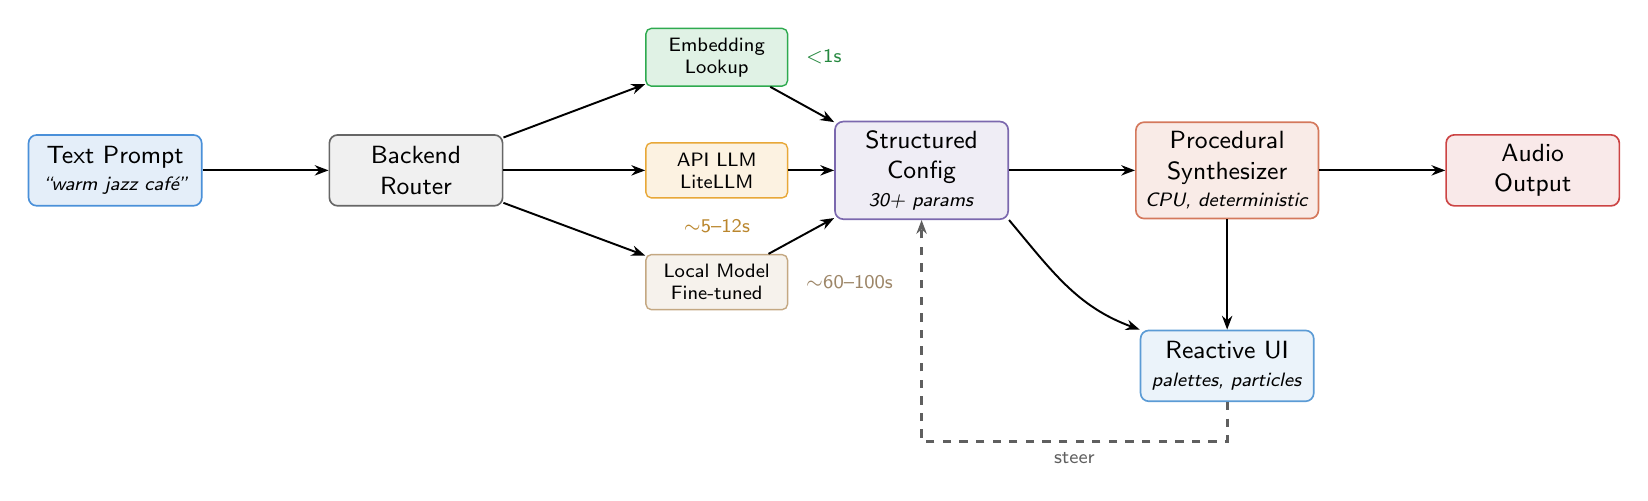
\begin{tikzpicture}[
    node distance=1.4cm and 1.8cm,
    >={Stealth[length=5pt]},
    box/.style={draw, rounded corners=3pt, minimum height=0.9cm, minimum width=2.2cm,
                font=\small\sffamily, align=center, line width=0.6pt},
    smallbox/.style={draw, rounded corners=2pt, minimum height=0.7cm, minimum width=1.8cm,
                     font=\scriptsize\sffamily, align=center, line width=0.5pt},
    arr/.style={->, thick, line width=0.7pt},
    darr/.style={->, dashed, thick, line width=1.0pt, color=steergray!70!black},
]

% Input
\node[box, fill=inputblue!15, draw=inputblue] (input) {Text Prompt\\[-1pt]\scriptsize\textit{``warm jazz caf\'{e}''}};

% Router
\node[box, fill=routergray!10, draw=routergray, right=1.6cm of input] (router) {Backend\\Router};

% Three backends
\node[smallbox, fill=embgreen!15, draw=embgreen, above right=0.6cm and 1.8cm of router] (emb) {Embedding\\Lookup};
\node[smallbox, fill=apiorange!15, draw=apiorange, right=1.8cm of router] (api) {API LLM\\{\scriptsize LiteLLM}};
\node[smallbox, fill=localtan!15, draw=localtan, below right=0.6cm and 1.8cm of router] (local) {Local Model\\{\scriptsize Fine-tuned}};

% Latency labels
\node[font=\scriptsize\sffamily\color{embgreen!80!black}, right=0.1cm of emb] {$<$1s};
\node[font=\scriptsize\sffamily\color{apiorange!80!black}, below=0.15cm of api] {$\sim$5--12s};
\node[font=\scriptsize\sffamily\color{localtan!80!black}, right=0.1cm of local] {$\sim$60--100s};

% Config
\node[box, fill=configpurple!12, draw=configpurple, right=4.2cm of router] (config) {Structured\\Config\\[-1pt]\scriptsize\textit{30+ params}};

% Synth
\node[box, fill=synthcoral!15, draw=synthcoral, right=1.6cm of config] (synth) {Procedural\\Synthesizer\\[-1pt]\scriptsize\textit{CPU, deterministic}};

% Audio output
\node[box, fill=audiored!12, draw=audiored, right=1.6cm of synth] (audio) {Audio\\Output};

% UI
\node[box, fill=uiblue!12, draw=uiblue, below=1.4cm of synth] (ui) {Reactive UI\\[-1pt]\scriptsize\textit{palettes, particles}};

% Arrows: input -> router
\draw[arr] (input) -- (router);

% Router -> backends
\draw[arr] (router) -- (emb);
\draw[arr] (router) -- (api);
\draw[arr] (router) -- (local);

% Backends -> config
\draw[arr] (emb) -- (config);
\draw[arr] (api) -- (config);
\draw[arr] (local) -- (config);

% Config -> synth -> audio
\draw[arr] (config) -- (synth);
\draw[arr] (synth) -- (audio);

% Config -> UI: smooth curve from config down-right to UI top-left
\draw[arr] (config.south east) to[out=-50, in=160] (ui.north west);

% Synth -> UI (audio features)
\draw[arr] (synth) -- (ui);

% Steering loop: wraps BELOW UI, then left and up into config bottom
\draw[darr] (ui.south) -- ++(0,-0.5)
    -| node[near start, below, font=\scriptsize\sffamily\color{steergray}] {steer} (config.south);

\end{tikzpicture}
\end{document}
